\documentclass[a4paper,12pt]{article}

%%%%%%%%%%%%%%%%%%%%
%%%%  PREAMBLE  %%%%
%%%%%%%%%%%%%%%%%%%%

\usepackage[T1]{fontenc}
\usepackage[utf8]{inputenc}

\usepackage[english,italian]{babel}

\usepackage{hyperref}
\hypersetup{hidelinks}

\usepackage[margin=2cm]{geometry}
\usepackage{minipage-marginpar}

\usepackage{enumitem}

\usepackage{graphicx}

\setlength{\parindent}{0em}
\setlength{\parskip}{1em}

\setlist[itemize]{itemsep=0.25em,topsep=0pt}
\setlist[enumerate]{itemsep=0.25em,topsep=0pt}

%%%%%%%%%%%%%%%%%%%%
%%%%  DOCUMENT  %%%%
%%%%%%%%%%%%%%%%%%%%

\title{Web Music Player}
\author{3 uomini e una $\lambda$}

\begin{document}

\maketitle
\newpage

\tableofcontents
\newpage

\section{Scopo del documento}

Il presente documento riporta l’analisi dei requisiti di sistema del progetto Web Music Player in linguaggio naturale. Lo scopo di questo di questo documento è quello di:
\begin{itemize}
    \item descrivere gli obiettivi del progetto
\end{itemize}

\section{Obiettivi del progetto}

Il progetto ha come obiettivo la realizzazione di una piattaforma online per l’ascolto di musica. Questo servizio deve offrire le funzionalità di un moderna piattaforma di streaming, focalizzandosi sull’utente e in particolare sulla proposta di nuova musica basata sui contenuti ascoltati.

Nello specifico, il servizio deve essere in grado di:

\begin{itemize}
    \item dare la possibilità ad un nuovo utente di registrarsi al suo primo accesso al sito web. Per la registrazione sono necessari un indirizzo email e una password. Una volta registrato l’utente può usufruire di una prova gratuita di 30 giorni prima di sottoscrivere un abbonamento  mensile. Un utente già registrato deve avere la possibilità di effettuare l’accesso tramite le sue credenziali;
    \item un utente dev’essere in grado di ricercare, ascoltare e riprodurre musica in streaming. Ha la possibilità di aggiungere alla Libreria canzoni, album e creare nuove playlist;
    \item presentare un’interfaccia web costituita da due schermate distinte, una barra superiore ed una barra inferiore. La schermata principale consiste nella Libreria dell’utente, ovvero dalle playlist create e da brani ed album salvati. La seconda è la schermata Scopri, il punto d’incontro tra utente e applicazione dove verrà proposta nuova musica. La barra superiore permette di passare da una schermata all’altra e di ricercare una canzone. La barra inferiore contiene le informazioni sul brano in riproduzione, permettendo di mettere in pausa, di passare alla canzone successiva e di modificare il volume;
    \item suggerire nuova musica sulla base dei gusti dell’utente. Questi vengono determinati dalle canzoni ascoltate, dai loro generi, dalle playlist create e dagli album salvati. L’utente deve essere in grado di interagire con le proposte, approvando i nuovi suggerimenti o rifiutandoli. In entrambi i casi, le decisioni vengono prese in considerazione per le future proposte.
\end{itemize}

\begin{figure}
    \centering
    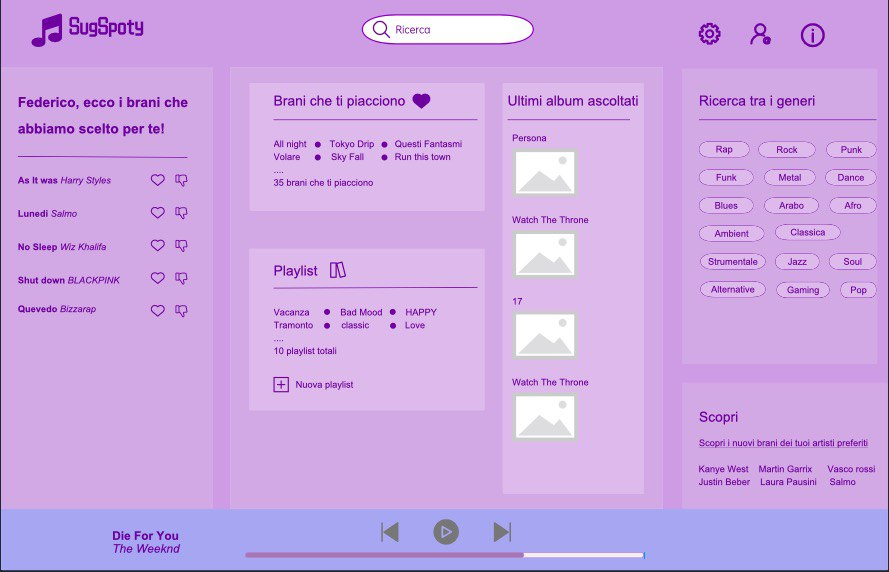
\includegraphics[width=\textwidth]{mock-up.jpg}
    \label{fig:mock-up}
    \caption{Mock-up}
\end{figure}

\end{document}